This chapter contains the fundamental concepts applied on this research.
Section~\ref{sec:bg-testing} presents the concepts related with Software
Testing. Section~\ref{sec:bg-codecoverage} describes the concept regarding code
coverage, which is the set of of components covered during the execution of test
cases. Debugging techniques based on code coverage, the basis of this research,
are detailed in Section~\ref{sec:bg-debugging}.
Finally, Section~\ref{sec:bg-infovis} covers the necessary concepts related with
the fields of Information Visualization and Human-Computer Interaction, both
necessary to conceive our novel metaphor, CodeForest.

\section{Testing}\label{sec:bg-testing}

This section presents the concepts defined by the Software Testing discipline
applied to automatic debugging strategies. Information generated during the
execution of tests enables the identification of failures and, thus, the search
for defects.

\subsection{Bugs everywhere}

No one knows when the first logical bug was introduced in a program; however, we
do know the exact day when the first actual bug was found in a computer. It was
a moth, found in the Harvard Mark II machine and eventually appended to a log
book by a technician (Figure~\ref{fig:firstbug}).
On September 9\superscript{th} 1947 the bug found its way into one of the 13,000
high-performance relays commissioned for this particular machine. Instantly
killed by the current, the remains of the insect made the machine fail. This
incident proved that computer problems could be caused by actual bugs.

\begin{figure}[h!]
\centering
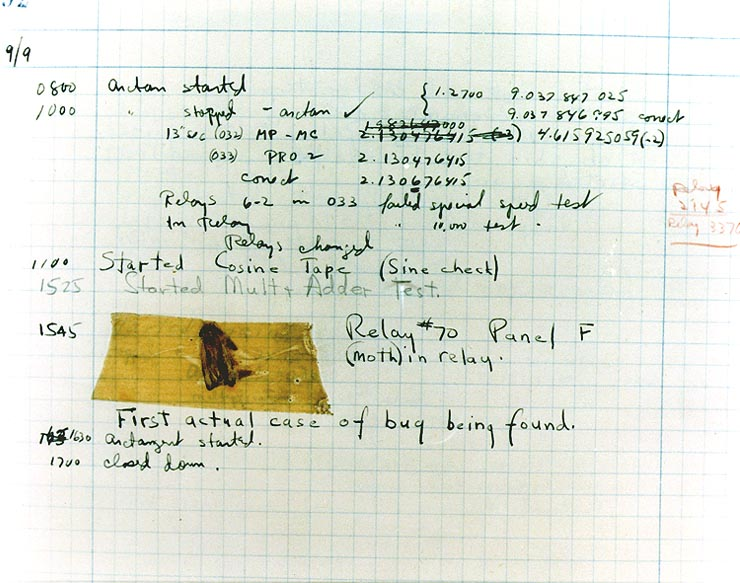
\includegraphics[width=1\textwidth]{figures/firstbug}
\caption{The first ``computer bug"\cite{naval1947bug}}
\label{fig:firstbug}
\end{figure}

The term gained popularity since that episode, causing software engineering
practitioners to use the term ``bug" to denote several things: an awry line of
code, a problematic state detected in runtime (for example, a wrong reference)
or an incorrect program execution (a program crashes in the presence of certain
inputs).
Despite being interconnected---one is a consequence of the other---lines of
code, program state, and execution output are elements separated in space and
time. Additionally, using a single term that assumes a different meaning
depending on the context clutters communication and favors confusion and
misunderstandings.

For this reason, it is important to disambiguate such situations.
Zeller \cite{zeller2009programs} proposes these terms:

\begin{itemize}
  \item \textit{A defect} denotes an incorrect piece of program code.
  \item \textit{An infection} denotes an incorrect program state.
  \item \textit{A failure} denotes an observable incorrect program behavior.
\end{itemize}

The IEEE Software and Systems Engineering
Vocabulary\footnote{\url{http://pascal.computer.org/sev_display/index.action}}
(\textit{SEVOCAB}) explains ``fault'' the same way as
``defect''\cite{zeller2009programs}. It also uses the term ``bug'' as a synonym
for ``fault'', which makes these terms equivalent.

The world where actual bugs could cause a failure lies in the past, along with
the original definition of debugging.
Since then, the term has been used to denominate the activity that locates and
corrects faults (defects) in a computer program using one or more techniques,
which can include the use of breakpoints, desk checking, dumps, inspection,
reversible execution, single-step operation, and traces. It is curious to notice
that this definition has not changed in twenty
years~\cite{ieee1990glossary,ieee2010vocabulary}.

Humphrey \cite{humphrey1999bugs} claims a psychological appeal in using the word
defect in detriment of bug. According to him, calling defects ``bugs'' usually
creates a tendency to minimize a potentially serious problem. For example, a
piece of software that gets to the end of Quality Assurance with ``a few bugs''.
When put this way, it does not sound so harmful. As scarier as it sounds,
defects are more like land mines than insects. Not all of them will explode, but
a few can be fatal, or at least very damaging.

\subsection{From defects to failures}\label{subsec:def-failure}

It takes four stages for a failure to happen. First, the developer introduces a
defect; that is,  a piece of code that can be the cause of an infection.
A defect turns into an infection when this specific piece of code is executed
under certain conditions that causes the infection. Once it takes place, the
program state differs from the one originally intended by the developer.
The propagation of the infection characterizes the third stage of a failure
lifecycle.
It is important to notice that an infection does not necessarily need to
propagate in a continuous fashion. It may be overwritten, masked, or corrected
later during program execution.
At the fourth stage, the infection causes a failure: an externally observable
error in the program behavior caused by an infection in the program state.

Thus, not every defect results in an infection, and not every infection results
in a failure. Also, having no failures does not imply having no defects.
Dijkstra pointed out that testing can only show the presence of defects, but
never their absence~\cite[p. 66]{buxton1970software}.

\subsection{From failures to fixes}

Having a failure as a starting point and working it until the defect is fixed is
an elaborate process, that demands certain steps to be followed. The first
letter of each step forms the TRAFFIC~\cite{zeller2009programs} acronym,
detailed in what follows.

\begin{enumerate}
  \item \textbf{T}rack the problem in the database.\label{list-1-traffic-track}
  \item \textbf{R}eproduce the failure.
  \item \textbf{A}utomate and simplify the test case.
  \item \textbf{F}ind possible infection origins.
  \item \textbf{F}ocus on the most likely origins.
  \item \textbf{I}solate the infection chain.
  \item \textbf{C}orrect the defect.
\end{enumerate}

Step 1---\textit{track the problem in the database}---states that all defects
must be tracked in a bug tracking tool (such as
Bugzilla\footnote{\url{http://www.bugzilla.org/}}). By centralizing all problems
in a single repository, management can use it as an asset, especially when it is
time to decide whether a system is ready for release. This is possible because
these tools classify defects by severity and priority. With the aid of a
bug tracking tool, one is able to find out which are the main problems and how
they can be avoided during development.

Step 2---\textit{reproduce the failure}---should be the first task of any
debugging activity, and it must occur exactly as stated in the original problem
report. The importance of this step is twofold: (1) if the defect cannot be
reproduced, there is only one alternative left---deduce from the source code what
might have happened to cause the problem; (2) to ensure that the problem is
fixed---if it is not possible to reproduce it, one can never affirm that the
problem has actually been fixed.

Step 3---\textit{automate and simplify the test case}. Once a problem has been
reproduced, it is time to simplify it.
The goal of this step is to find out, for every circumstance associated with the
defect, whether it is relevant---something that is absolutely required to make
the problem occur---or not. A circumstance is any aspect that may influence the
problem. The outcome of this step is a test case containing only the relevant
circumstances to recreate the failure. By doing so, it is also possible  to
track duplicated failure reports registered in a bug tracking tool.

Steps 4, 5 and 6---respectively \textit{find possible infection origins, focus
on the most likely origins, and isolate the infection chain}---are the most
resource-consuming steps of the process. Understanding the failure is a
difficult task because it demands a two-dimensional analysis through spatial and
temporal dimensions.
The spatial dimension refers to  where the infection takes place in the source
code. The temporal dimension determines when  the failure happens during the
program execution. The examination of space and time are demanding tasks for
even  simple programs because each state can comprise several variables.

Step 7---\textit{correct the defect}---should be the simplest of all steps; when
it is reached, it is expected that the developer has full comprehension of the
failure. In order to consider a failure as ``fixed'', three concerns must be
addressed by the developer.
\begin{itemize}
  \item \textit{Does the failure no longer occur?} One must ensure that the
  correction makes the failure no longer occur. This requires
  clarification since there are two ways of fixing a failure: by correcting its
  root cause or by correcting an infectious state. The former ensures that
  the defect will not happen again while the latter does not offer the same
  guarantee.
  \item \textit{Did the correction introduce new problems?} This can be
  difficult to verify when there is no automated regression test suite available.
  \item \textit{Was the same mistake made elsewhere?} One must check for
  possible defects that may be caused by the same mistake.
\end{itemize}

\section{Code coverage}\label{sec:bg-codecoverage}
Code coverage---also known as \textit{program spectra}
\cite{renieris2003,harrold1998,dickinson2001}---can be defined as a set of
components covered during the execution of test cases \cite{elbaum2001}.
Components in this context are statements, predicates, def-use associations or
function calls~\cite{Abreu2008}.

Therefore, code coverage is associated with dynamic verification of control
and/or data flows occurring  during the execution of a program. It can be
associated with unit (intraprocedural) coverage or integration
(interprocedural) coverage. In what follows, we discuss the different types of
code coverage.

\subsection{Unit coverage}

Consider the program presented in Figure~\ref{fig-max}  which determines the
maximum element in an array of integers.  The lines of code  associated
with the statements of the program are presented. The program has a defect
localized in line 2.

Typically, a program $ P $ is mapped into a flow graph  $G(N,E, s, e)$
where $N$ is the set of blocks of statements (nodes) such that once
the first statement is executed all statements are executed in
sequence, $s$ is the start node, $e$ is the exit node, and $E$ is
the set of edges ($n'$,$n$), such that $n' \neq n$, which represents a possible transfer of
control between node $n'$ and node $n$ \cite{chaim2013}. Figure~\ref{fig-gfcMax} contains the flow
graph obtained from program max; and Figure~\ref{fig-max} lists the statements associated with each node.

\begin{figure}[h!]
\centering
\begin{tabular}{|c|c|c|l|}
  \hline Line & Statement & Node & Code \\
  \hline
  1 & - & - & int max(int array [], int length) \\
  2 & - & 1 & \{ \\
  3 & 1 & 1 & \hspace{0.2 cm} int i = 0; \\
  4 & 2 & 1 & \hspace{0.2 cm} int max = array[++i]; \textbf{//array[i++];} \\
  5 & 3 & 2 & \hspace{0.2 cm} while(i $<$ length) \\
  6 & - & 3 & \hspace{0.2 cm} \{ \\
  7 & 4 & 3 & \hspace{0.6 cm} if(array[i] $>$ max) \\
  8 & 5 & 4 & \hspace{1.0 cm} max = array[i]; \\
  9 & 6 & 5 & \hspace{0.6 cm} i = i + 1; \\
  10 & - & 5 & \hspace{0.2 cm} \} \\
  11 & 7 & 6 & \hspace{0.2 cm} return max; \\
  12 & - & 6 & \} \\
  \hline
\end{tabular}
\caption{Example program \textit{max} \cite{chaim2013}.\label{fig-max}}
\end{figure}

\begin{figure}
  \centering
    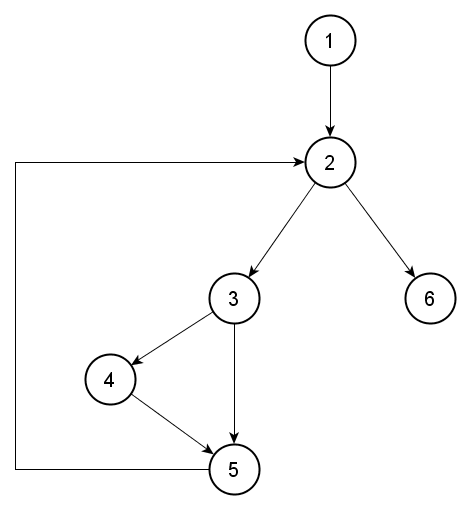
\includegraphics[height=8cm]{figures/gfcMax.png}
  \caption{Control-flow graph for program \textit{max}.}
  \label{fig-gfcMax}
\end{figure}


A brief explanation of  the different types of code
coverage is presented below.

\begin{itemize}
  \item \textit{Statement coverage} identifies the statements traversed by a
    single test case or test suite.

  \item \textit{Node coverage} refers to nodes
    exercised by test cases.   Statement and node coverage are similar. The
    difference  may arise when, for example, conditional assignments are present
    in a statement since there are more than one node in such statements
    \cite{souza13adding}. A test set that satisfies the node coverage always
    satisfies the statement coverage. The opposite is not always true.

  \item \textit{Predicate coverage} identifies predicate commands traversed by
    the test case. A predicate is a boolean expression referring to
    some property present in some point of the program~\cite{zhang2009non}.
    Predicate commands are associated with a condition verified during an
    execution, in which a deviation in the control flow can occur, such as
    in \textit{if} and \textit{while} commands. For example, there are
    predicates in lines 3 and 4 of program \textit{max}.
\end{itemize}

To illustrate the  coverage regarding program \textit{max}, consider
Table~\ref{tab-casoteste-tarantula}. It presents five test cases ($t_1, t_2$,
$t_3$, $t_4$, and $t5$) to test  \textit{max}. When executed, test cases $t_4$
and $t_5$ fail, while $t_1, t_2$, and $t_3$ pass.

\begin{table}
\center
\caption{Test cases for program \textit{max}.\label{tab-casoteste-tarantula}}
\begin{tabular}{c|l|c|c}
\hline $T_n$ & Input data & Expected Outcome & Actual Outcome\\
\hline $t_1$ & max( [1,2,3] , 3 ) & 3 & 3\\
\hline $t_2$ & max( [5,5,6] , 3 ) & 6 & 6\\
\hline $t_3$ & max( [2,1,10] , 3 ) & 10 & 10\\
\hline $t_4$ & max( [4,3,2] , 3 ) & 4 & 3\\
\hline $t_5$ & max( [4] , 1 ) & 4 & error\\
\hline
\end{tabular}
\end{table}

Table~\ref{tab-cov} presents the statement and node coverage for each test case.
The bullet associated with each statement, node and test case means that the
particular test case exercises during testing these components.
Table~\ref{tab-cov-predicate} presents predicate coverage.  Note that each
predicate has two outcomes: true or false. A test case may execute both outcomes
or only one of them.

Coverages based on the program data-flow are also used for debugging purposes
\cite{santelices09dataflow,chaim04DRT}. Definition-use associations (duas)
\cite{rapps85dataflow}, which involves a definition of a variable (an
assignment of value) and its subsequent use (a reference to this value), is an
example of data-flow coverage. Since our goal is to address the visualization
of debugging information obtained from unit and integration control-flow
coverages, data-flow coverages are out of the scope of this work.

\begin{table}
\center
\caption{Statement and node coverage of program \textit{max}.\label{tab-cov}}
\begin{tabular}{|c|c||c|c|c|c|c|}
  \hline Line & Node &$t_1$ & $t_2$ & $t_3$ & $t_4$ & $t_5$  \\
  \hline  3 & 1 & $\bullet$ & $\bullet$ & $\bullet$ & $\bullet$ & $\bullet$  \\
  \hline  4 & 1 & $\bullet$ & $\bullet$ & $\bullet$ & $\bullet$ & $\bullet$  \\
  \hline  5 & 2 & $\bullet$ & $\bullet$ & $\bullet$ & $\bullet$ &   \\
  \hline  7 & 3 & $\bullet$ & $\bullet$ & $\bullet$ & $\bullet$ &   \\
  \hline  8 & 4 & $\bullet$ & $\bullet$ & $\bullet$ &           &   \\
  \hline  9 & 5 & $\bullet$ & $\bullet$ & $\bullet$ & $\bullet$ &   \\
  \hline 11 & 6 & $\bullet$ & $\bullet$ & $\bullet$ & $\bullet$ &   \\
  \hline  - & - & Pass & Pass & Pass & Fail & Fail  \\
  \hline
\end{tabular}
\end{table}

\begin{table}
\center
\caption{Predicate coverage of program \textit{max}.\label{tab-cov-predicate}}
\begin{tabular}{|c|c|c|c|c|c|c|}
\hline \multicolumn{2}{|c|}{Predicate} &\multirow{2}{*}{$t_1$} & \multirow{2}{*}{$t_2$} & \multirow{2}{*}{$t_3$} & \multirow{2}{*}{$t_4$} & \multirow{2}{*}{$t_5$}  \\
  \cline{1-2} Line & Outcome & &  &  &  &   \\
  \hline 5 & true & $\bullet$ & $\bullet$ & $\bullet$ & $\bullet$ &    \\
  \hline 5 & false & $\bullet$ & $\bullet$ & $\bullet$ & $\bullet$ &  \\
  \hline 7 & true & $\bullet$ & $\bullet$ & $\bullet$ &  &   \\
  \hline 7 & false & $\bullet$ & $\bullet$ & $\bullet$ & $\bullet$  &   \\
  \hline - & - & Pass & Pass & Pass & Fail & Fail  \\
  \hline
\end{tabular}
\end{table}
\subsection{Integration coverage}
The aforementioned coverages are obtained by testing the unit, being a unit a
method of a program\footnote{The term \textit{method} is utilized to refer to a
module (e.g., procedure, function, method) in a program.}. Nevertheless,
coverages related to integration testing data can also be used for debugging
purposes.

A typical integration coverage is \textit{module or call function coverage}
which reports the modules (e.g., procedures, functions, or methods) exercised
by a test case or suite. In this work, we utilize the \textit{MethodCallPair}
(MCP) integration coverage which was proposed by Souza
\cite{souza2012depuracao,souza13adding} and is described as follows.

The \textit{MethodCallPair} (MCP) integration coverage was developed to collect
information about the most suspicious method call sequences. MCP was not devised
as a testing requirement. Rather, it was conceived as integration information
captured during test suite execution for debugging purposes.

MCP represents pairs of methods exercised during a test suite run. A pair is
composed of a \textit {caller} method and a \textit{callee}  method. Instead of
simply capturing the method call stack to calculate their suspiciousness, the
\textit{rationale} is to highlight methods more often related to other methods
in failed executions. Thus, the integration between methods is used to indicate
those more likely to contain faults.
Figure~\ref{fig:mcp} illustrates MCP coverage information in which the method
\textit{caller} of the class \textit{A} invokes the method \textit{callee} of
the class \textit {B}.

%switch this figure for a tikz figure
\begin{figure}[h]
  \centering
  \scalebox{.40}{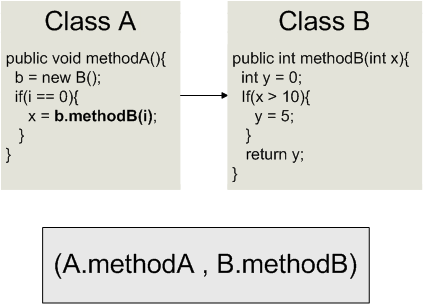
\includegraphics{figures/fig-DCI_MCP.png}}
  \caption{MethodCallPair (MCP).}
  \label{fig:mcp}
\end{figure}

Several techniques utilize heuristics that are based on the execution frequency
of nodes, statements, predicates and MCPs to find out the ones that are more
suspicious to contain defects~\cite{souza2012depuracao}.

The following section presents further details on how code coverage information
is used to support debugging activities, which will provide the foundations for
our novel metaphor, called CodeForest.

\section{Coverage based debugging}\label{sec:bg-debugging}

\newcommand{\bl}{%
$\bullet$
}
Code coverage information is utilized by heuristics to calculate the
suspiciousness of components. After assigning a suspiciousness value to these
components, a classification list of components in descending order of
suspiciousness is generated.

Thus, the heuristics used to elect suspicious excerpts of code are a pivotal
issue in coverage based debugging. Several heuristics have been proposed or
utilized to indicate components (statements, predicates, def-use associations,
methods or MCPs) most likely to contain faults. Ranking
heuristics---characterized by identifying suspicious code excerpts from the
frequency of executed components in passing and failing test cases---are
prevalent.
There are ranking heuristics created specifically for fault localization
\cite{jones2002visualization,Wong2007}, while others have been adapted from
areas such as Molecular Biology \cite{Abreu2007,gonzalez2007}.

In what follows, debugging techniques based on code coverage are described.
Firstly, techniques that utilize unit code coverage are presented, then the use
of integration coverage in fault localization is discussed.

\subsection{Unit coverage debugging}

The \textit{Tarantula} heuristic~\cite{jones2002visualization} is one of the first ranking
heuristics utilized to assign suspiciousness values to program statements. For
each component, Tarantula calculates the frequency that a component is executed
in failing test cases and divides it by the frequency that this
component is executed in failing and passing test cases.

Tarantula's formula $H_{T}$ is shown below in Equation~\ref{eq:tarantula}:
$c_{ef}$ indicates the number of times that a component ($c$) is executed ($e$)
in failing ($f$) test cases, $c_{nf}$ is the number of times that a
component is not ($n$) executed in failing ($f$) test cases,
$c_{ep}$ is the number of times that a component is executed ($e$) by a
passing ($p$) test case and $c_{np}$ represents the number of times
that a component is not ($n$) executed by passing ($p$) test
cases.

\begin{equation} \label{eq:tarantula}
 H_{T} = \frac{\frac{c_{ef}}{c_{ef} + c_{nf}}}{\frac{c_{ef}}{c_{ef} + c_{nf}} + \frac{c_{ep}}{c_{ep} + c_{np}}}
\end{equation}



Table~\ref{tab-cov-tarantula} presents the statement and node coverage, the
outcome of each test presented in Table~\ref{tab-casoteste-tarantula}  and the
values of the coefficients utilized to determine the suspiciousness using
Tarantula. The suspiciousness value for lines 3 and 4 is 0.5 and for the rest of the lines
is 0.33 or 0. Therefore, lines 3 and 4 (i.e., node 1) are the most suspicious
statements according to Tarantula. Other heuristics utilize the
same coefficients with different formulae to determine the suspiciousness values.

\begin{table}
\center
\caption{Statement and node coverage of program \textit{max}.\label{tab-cov-tarantula}}
\begin{tabular}{|c|c|c|c|c|c|c|c|c|c|c|c|c|}
 \hline Line & Statement & Node &$t_1$ & $t_2$ & $t_3$ & $t_4$ & $t_5$ &
 $c_{np}$ & $c_{ep}$ & $c_{nf}$ & $c_{ef}$ & $H_{T}$ \\
 \hline 1 & - & - & \bl & \bl & \bl & \bl & \bl & 0 & 3 & 0 & 2 & 0.5\\
 \hline 2 & - & 1 & \bl & \bl & \bl & \bl & \bl & 0 & 3 & 0 & 2 & 0.5\\
 \hline 3 & 1 & 1 & \bl & \bl & \bl & \bl & \bl & 0 & 3 & 0 & 2 & 0.5\\
 \hline 4 & 2 & 1 & \bl & \bl & \bl & \bl & \bl & 0 & 3 & 0 & 2 & 0.5\\
 \hline 5 & 3 & 2 & \bl & \bl & \bl & \bl &     & 0 & 3 & 1 & 1 & 0.33\\
 \hline 6 & - & 3 & \bl & \bl & \bl & \bl &     & 0 & 3 & 1 & 1 & 0.33\\
 \hline 7 & 4 & 3 & \bl & \bl & \bl & \bl &     & 0 & 3 & 1 & 1 & 0.33\\
 \hline 8 & 5 & 4 & \bl & \bl & \bl &     &     & 0 & 3 & 2 & 0 & 0\\
 \hline 9 & 6 & 5 & \bl & \bl & \bl & \bl &     & 0 & 3 & 1 & 1 & 0.33\\
 \hline 10 & - & 5 & \bl & \bl & \bl & \bl &     & 0 & 3 & 1 & 1 & 0.33\\
 \hline 11 & 7 & 6 & \bl & \bl & \bl & \bl &     & 0 & 3 & 1 & 1 & 0.33\\
 \hline 12 & - & 6 & \bl & \bl & \bl & \bl &     & 0 & 3 & 1 & 1 & 0.33\\
  \hline - & - & - & Pass & Pass & Pass & Fail & Fail & - & - & - & - & - \\
  \hline
\end{tabular}
\end{table}

\subsection{Integration coverage debugging}

A limitation of the current ranking heuristics is the lack of guidance to search
for faults in larger portions of code since they assign suspiciousness values
only to statements. Parnin and Orso \cite{parnin2011automated} performed experiments with
a group of developers using Tarantula and observed that  developers take into
account their knowledge of the code to search for faults without usually
following Tarantula's classification. In this sense, the results suggest that
contextual guidance might be helpful to coverage based debugging.

We discuss below two approaches that utilize integration coverage to provide
contextual support in the search for bugs.

\subsubsection{Code hierarchy}

Souza~\cite{souza2012depuracao} proposed a search heuristic called \textit{code
hierarchy} (CH) that attributes suspiciousness values to packages, classes and methods. The CH
suspiciousness value is given by a pair (\textit{susp}, \textit{number}) where
\textit{susp} is the highest suspiciousness value assigned to a node belonging
to the program entity (package, class or method) and \textit{number} is the
number of nodes which has that suspiciousness value.

Algorithm~\ref{alg-CH} shows how the CH value is assigned to classes. It
requires that the suspiciousness values of the nodes be previously determined.
From now on, the suspiciousness values assigned to nodes are determined by
utilizing Tarantula, although any other ranking heuristic
\cite{Wong2007,Abreu2007,gonzalez2007} can be used as well. The algorithms to
calculate CH values to packages and methods are similar.


Packages, classes, and methods are firstly ordered by their \textit{susp}
value and then inversely by the \textit{number} value. CH
establishes that the \textit{susp} value is the most important factor for fault
localization. Thus, if a method has only one node with the highest
suspiciousness value, it should be investigated first. In case of a draw, the
number of nodes with the same \textit{susp} value decides which is the next
entity to be investigated. The smaller the ``number'', the better. In case of a
double draw, the next entity is decided randomly.

%code hierarchy
\begin{algorithm}
\KwIn{A list of nodes and a list of classes (\textit{node\-List}, \textit{classList})}
\KwOut{A list of classes with CH values (\textit{susp}, \textit{number})
assigned}
\BlankLine

\ForEach{$class$ \textbf{in} $classList$}
{
  \ForEach{$node$ \textbf{in} $nodeList$}
  {
    \If{$node$.class = $class$}{
      \If{$node$.susp $>$ $class$.susp}{
    $class$.susp $\leftarrow$ $node$.susp\;
    $class$.number $\leftarrow$ 1\;
      }
      \ElseIf{$node$.susp = $class$.susp}{
    $class$.number++\;
      }
    }
  }
}
\Return{$classList$}\;
\caption{Assignment of CH values to classes}
\label{alg-CH}
\end{algorithm}

In our visual representation of programs, we utilize CH suspiciousness values
to determine the positioning and coloring of packages, classes, and methods.

\subsubsection{Creating roadmaps for fault localization}

Souza~\cite{souza2012depuracao} proposed  to add contextual information to
support fault localization by creating roadmaps from the ranking of the MCP
coverage.  The roadmap, referred to as R-MCP, is a simplified guide to be used
when searching for faults. It is determined according to the following steps.
\begin{enumerate}
\item Pairs of methods (MCPs) are tracked during the execution of each test case.
\item MCP coverage collected during the test suite execution is used to assign
suspiciousness values to each MCP.  Any ranking heuristic can be used with this purpose. In the case of using Tarantula,  coverage data regarding pairs of methods (MCPs) are  the components  of the  formula presented in Equation~\ref{eq:tarantula}. % We have chosen to use Tarantula because it was one of the first ranking heuristics proposed; nevertheless, any other heuristic could have been used as well.
\item A list of MCPs sorted by suspiciousness is created. MCPs with the same suspiciousness values are sorted by their  order of occurrence in the execution.
\item R-MCP is created by visiting  the MCP list from the top ranked elements to the least ranked ones, and from the caller method to the callee method. The caller method  and the callee method of each visited pair  is verified in this order. If a method is not yet in the roadmap, it is  added to it with the same suspiciousness value assigned to the visited pair. Thus, the roadmap contains each method executed in the test suite with its highest suspiciousness in the MCP  list.

\end{enumerate}

Consider that an MCP (\textit{A.methodA},\textit{B.methodB}) is executed in 4
out of 10 test cases that fail and it is executed only in 2 test cases that pass
in a total of 90 successful test cases. Thus,  coefficients $c_{ef}$, $c_{nf}$,
$c_{ep}$, and $c_{np}$ of  equation~\ref{eq:tarantula} will be, respectively, 4,
6, 2, and 88. As a result, the Tarantula suspiciousness value ($H_T$) will be
0.941 for MCP (\textit{A.methodA},\textit{B.methodB}).  Once all MCPs have been
assigned  their $H_T$, they are sorted in decreasing order; the list of sorted
MCPs is then used to create the roadmap. During R-MCP creation, if
\textit{A.methodA} is  not in the roadmap yet, it is inserted in  R-MCP with
assigned suspiciouness 0.941. Next,  \textit{B.methodB} is checked. If not yet
in R-MCP, \textit{B.methodB} is also inserted with suspiciousness 0.941.

The rationale to create R-MCP is based on a developer using a sorted MCP list to
search for faults: the developer looks at the top MCP of the list and examines
the  caller method. If it does not contain the bug, he/she looks at the callee
method.  If the bug is not discovered by visiting the methods of the top MCP,
the search proceeds by inspecting the methods of the following MCPs.
When checking an MCP, if a method is seen anew, the developer does not inspect
the method again. Instead, he/she skips the method and proceeds with the next
not inspected method until finding the bug.

Therefore, R-MCP is composed of each method in the MCP list with its highest
suspiciousness value. Methods that appear in more than one pair in the MCP list
are included only once in R-MCP. Thus, by  using R-MCP, methods are not checked
repeatedly. Table~\ref{tab:rmcp-commons} presents an example of R-MCP generated
for a faulty version of the Apache Commons-Math program
\cite{souza2012depuracao}.

\begin{table}[h]
\center
  \caption{R-MCP roadmap for Commons-Math AE\_AK\_1 bug.}
  \label{tab:rmcp-commons}
  \begin{tabular}{l|r}
    \hline \textbf{method} & \textbf{suspiciousness} \\
    %\arrayrulecolor{black}
    \hline %\rowcolor[cmyk]{0.3,0.1,0,0}
    {getCovariances} & {$0.9985037$} \\
    \hline getAllParameters & $0.9985037$ \\
    \hline getMeasurements & $0.9985037$ \\
    \hline EstimatedParameter & $0.997012$ \\
    \hline getName & $0.9960199$ \\
    \hline solve & $0.9955246$ \\
    \hline buildMessage & $0.9955246$ \\
    \hline MathException & $0.9955246$ \\
    \hline EstimationException & $0.9955246$ \\
    \hline updateJacobian & $0.9950298$ \\
    \hline GaussNewtonEstimator & $0.9930556$ \\
    \hline estimate & $0.9930556$ \\
    \hline SimpleEstimationProblem & $0.9930556$ \\
    \hline getUnboundParameters & $0.9930556$ \\
    \hline addParameter & $0.9930556$ \\
    \hline addMeasurement & $0.9930556$ \\
    \hline
  \end{tabular}
\end{table}

The R-MCP's underlying intuition is that the developer will start the
exploration of the code by the top ranked methods. When visiting a particular
method, he/she will resort to unit coverage debugging to investigate the method.
In debugging Commons-Math bug  AE\_AK\_1, the developer would start by the
method \textit{getCovariances()} and then move to the next ones until finding
the bug site. In failing to do so, the developer will need to resort to another
debugging technique.

In most cases, a method is composed of nodes that are classified with different
suspiciousness values.
The delta suspiciousness ($\Delta_{s}$) is a strategy proposed to deal with this
issue. The idea is  to investigate nodes with suspiciousness values slightly
lower than the method suspiciousness. The aim is to include  the bug in the set
of nodes to be investigated without growing excessively the number of nodes to
examine.

Thus, a developer will inspect nodes with suspiciousness values equal to or
greater than $\Delta_{s}$. The formula of $\Delta_{s}$ is shown in
Equation~\ref{eq-delta}. $M_{s}$ is the method suspiciousness value and $p$ is
the percentual value used.

\begin{equation}
\label{eq-delta}
 \text{$\Delta_{s}$} = M_s * (1 - p)
\end{equation}

Souza and Chaim~\cite{souza13adding} showed that by using $\Delta_{s}$ with $p =
3\%$ less code is investigated in comparison to a strategy using Tarantula and
node coverage. In debugging Commons-Math bug  AE\_AK\_1, only nodes with
suspiciousness $0.9985037 (1-0.03)$, i.e., $0.96854859$, will be investigated
during the exploration of \textit{getCovariances()} with the delta suspiciousness
strategy. By doing so, the authors expect to reduce the number of inspected
nodes by visited method.

In Chapter~\ref{ch:forest}, we will present how the suspiciousness values of
nodes, methods, and classes are mapped into a visual metaphor. The
implementation of the R-MCP roadmap in the plugin for fault localization based
on the visual metaphor is discussed in Chapter~\ref{ch:plugin}.

In what follows, the concepts regarding information visualization are described.

\section{Information visualization}\label{sec:bg-infovis}

The field of visualization is concerned with the mapping of data to pixel values
in such a way that meaningful conclusions about the data can be
drawn~\cite[p.~397]{erik2008color}. The essence of this definition includes the
analyst, user interfaces, graphics and data \cite{myatt2009making}.

The research field of visualization can be split into two major areas.
\textit{Scientific visualization} is primarily concerned with the visualization
of multi-dimensional phenomena---architectural, meteorological, medical,
biological, etc. \textit{Information visualization} is primarily concerned with
the visualization of large-scale collections of non-numerical information, such
as large networks, hierarchies, data bases, text, etc. Presenting abstract data,
especially very-large scale, still poses a continuing
challenge~\cite{friendly2001milestones}.

Statistical graphics and data visualization, despite common belief, are far from
being a modern development in statistics. It is possible to trace the art of
portraying quantitative information back in time, into the histories of the
earliest map-making and visual depiction, and later into thematic cartography,
statistics and statistical graphics~\cite{friendly2008brief}.

Visual information, when well organized and arranged in a structured way, is
capable of elevating our comprehension levels about some information. It is more
effective to use colors, shapes and textures---and other visual techniques---to
convey information when compared to a text-only approach.

\subsection{Interface metaphors}

According to Lakoff and Johnson, a metaphor is ``understanding and experience
one kind of thing in terms of another''. Metaphors are not only pervasive in
language, but they are a fundamental part of our conceptual system of thought
and action~\cite{lakoff1980metaphors}. They are so important in our lives
that there is a proposition that all knowledge is based on
metaphors~\cite{indurkhya1994thesis}.

The field of Human-Computer Interaction conceives metaphors as cross-domain
mappings, with the goal of allowing the transference (or mapping) of knowledge
from a source domain (a familiar area of knowledge) to a target domain
(unfamiliar area or situation). This enables humans to use specific prior
knowledge and experience for understanding and behaving in situations that are
novel or unfamiliar~\cite{helander1997handbook}.

An interface metaphor is a set of user interface visuals, actions and procedures
that exploit specific knowledge that users already have of other domains. The
purpose is to give users instantaneous knowledge about how to interact with the
user interface. It helps establish expectations and encourage predictions about
system behavior. A well known example is the use of the ``desktop'' metaphor on
computers. It portrays an Operating System as objects, tasks and behaviors found
in physical office environments. The ``Trashcan'' found on the Windows Desktop
quickly helps users understanding the concept of deletion of files.

The problem with metaphors starts when these comparisons are taken too far. A
good example is the first generation of word processors, which heavily relied on
the typewriter metaphor. It is a fact that the keyboard of a computer closely
resembles the one found in a standard typewriter, and so it seemed like a good
metaphor to use. The space key in a typewriter is not a character, it just moves
the guide further along the current line. In a word processor, the space is a
character, inserted within a text just as any character is inserted.
This is the point where the metaphor gets in the way of the user understanding a
word processor~\cite{dix2004human, helander1997handbook}.

Other precautions must be taken when dealing with metaphors. Do not assume that
a given metaphor is free of cultural bias, i.e, not every metaphor is universal.
Also, the number of visual representations provided by the metaphor should be
sufficient to cover all objects in the chosen domain. Although possible, it is
not advisable to combine representations from different
metaphors~\cite{diehl2007software}.

\subsection{Visual encoding}

The mechanism of vision is intricate and its study is out of the the scope of
this research. But in order to better understand the principles that have guided this
work, we need to introduce a few concepts regarding the vision mechanism. In
fact, we do not see with our eyes; we see with our brains. Our eyes work as
complex sensory mechanisms through which light enters. Then, the light is
translated into electrical impulses that are passed on to and around our brains.
It is in our brain that occurs the process of making sense of what our eyes
register actually happens.

Without the filters and limits present in our eyes, the excessive amount of
information captured could easily overwhelm our brains. For this reason, our
eyes only register what lies within their span of perception. This small portion
of what our eyes sense will then become an object of focus. An even smallest
fraction of that portion will capture our attention or conscious
thought~\cite{wandell1995foundations}.

One of the several stages that happens in our brain when performing the vision
process is called ``preattentive processing''.
It is one of the early stages of visual perception that rapidly occurs below the
level of consciousness. This process is oriented to detect a specific set of
visual attributes.
A series of experiments conducted on this subject~\cite{treisman1988feature}
studied the reaction time of an individual searching for a particular shape
(called target) when presented in a set of other shapes (called distracters).
The main finding was that, for certain combinations of targets and distracters,
the time to find the target \textit{did not} depend on the number of
distracters, suggesting that this processing happens in a parallel and automatic
fashion.

In his book, Ware~\cite{ware2008visual} suggests seventeen ``preattentive''
attributes. The most relevant ones were narrowed down
in~\cite{few2006information}, and are shown in Figure~\ref{fig:preattentive}.
These attributes are perceived within 200 milliseconds, i.e., the time interval
it takes before the eye reacts and moves~\cite{healey1996high}.

\begin{figure}[h!]
\centering
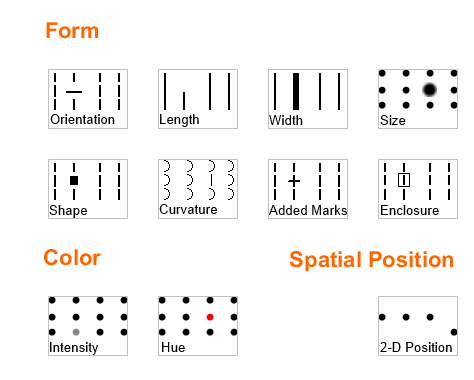
\includegraphics[width=1\textwidth]{figures/ali-encodings}
\caption{Interpretation of Few's preattentive attributes\cite{few2006information}}
\label{fig:preattentive}
\end{figure}

After the stage of feature extraction is done, the stage of pattern perception
takes place. At this point, the brain starts the segmentation of the visual
world into distinct regions to discover the structure of objects and the
connections between them. At the third and final stage, the brain does attentive
processes to perform the analytical task at hand.

With this information in mind, we believe that an effective way of conveying
information is the one that exploits the first stage of this mechanism, by
letting the preattentive processing do some thinking on our behalf.
Although it is not a straightforward process due to the fact that the
effectiveness of these attributes strongly varies based on the desired data type
to encode, there are some ``rules of thumb'' that can be
applied~\cite{mackinlay1986automating}.
Table~\ref{tab:mackinlay} presents a ranking showing the effectiveness as a
function of the data type. It is important to notice that picking the most
effective encodings relies heavily on the task at hand, so even the encoding
rankings should be seen in that light. It is also possible to encode a data type
within more than one visual channel, in order to help perform the task more
effectively~\cite{thoughtworks2012thoughtworks}.

\begin{table}[!ht]
    \centering
    \caption{Mackinlay's rankings~\cite{mackinlay1986automating}}
    \begin{tabular}{ c c c }
    \textbf{Quantitative} & \textbf{Ordinal} & \textbf{Nominal} \\
    \hline\hline
    Position     & Position    & Position    \\
    Length       & Density     & Hue         \\
    Angle        & Saturation  & Texture     \\
    Slope        & Hue         & Connection  \\
    Area         & Texture     & Containment \\
    Volume       & Connection  & Density     \\
    Density      & Containment & Saturation  \\
    Saturation   & Length      & Shape       \\
    Hue          & Angle       & Length      \\
    Texture      & Slope       & Angle       \\
    Connection   & Area        & Slope       \\
    Containment  & Volume      & Area        \\
    Shape        & Shape       & Volume      \\
    \hline
    \end{tabular}
\label{tab:mackinlay}
\end{table}

A domain set is \textit{quantitative} when it is a range, such as $[1,2,3,4,5]$;
it is \textit{ordinal} when it is an ordered tuple, such as $\langle{}Monday,
Tuesday, Wednesday\rangle{}$; and it is \textit{nominal} when there is the
absence of a relation of order among elements, such as\newline
$\{Marcos, Higor, Danilo\}$.
Figure~\ref{fig:energy2012short} presents a comparison between two quantitative
pieces of data: the American national average monthly gasoline retail price and
the monthly residential electricity price~\cite{energy2012short}. The figure
makes use of the following Mackinlay attributes: position, angle, slope, area,
color hue, connection and containment.

\begin{figure}[H]
\centering
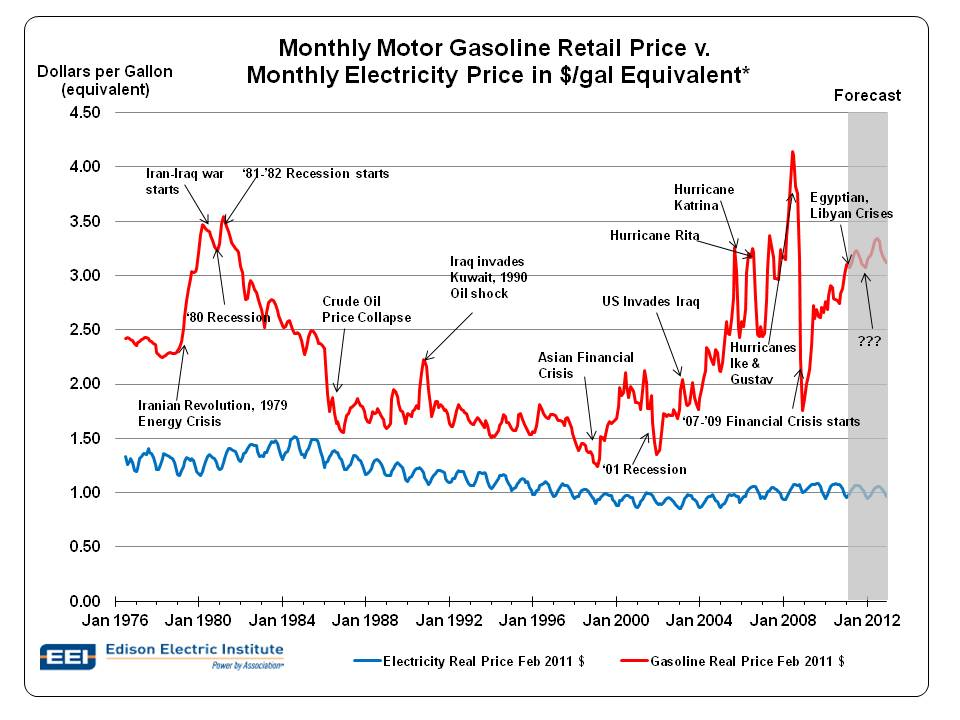
\includegraphics[width=.6\textwidth]{figures/energy2012short}
\caption{National average monthly gasoline retail price versus \\ monthly residential electricity
price~\cite{energy2012short}}
\label{fig:energy2012short}
\end{figure}

Figure~\ref{fig:citc2013organizational} presents the Saudi Arabian
Communications and Information Technology Commission organizational structure,
as an example of a ordinal set. The purpose of a organizational chart is to show
the structure of an organization and the relationships and relative ranks of its
parts and position/jobs. There is a clear distinction of which position is above
or under or equivalent to which, and who is the head of the organization. The
figure makes use of the following Mackinlay attributes: position, color hue,
connection, containment, length, area, and shape.

\begin{figure}[H]
\centering
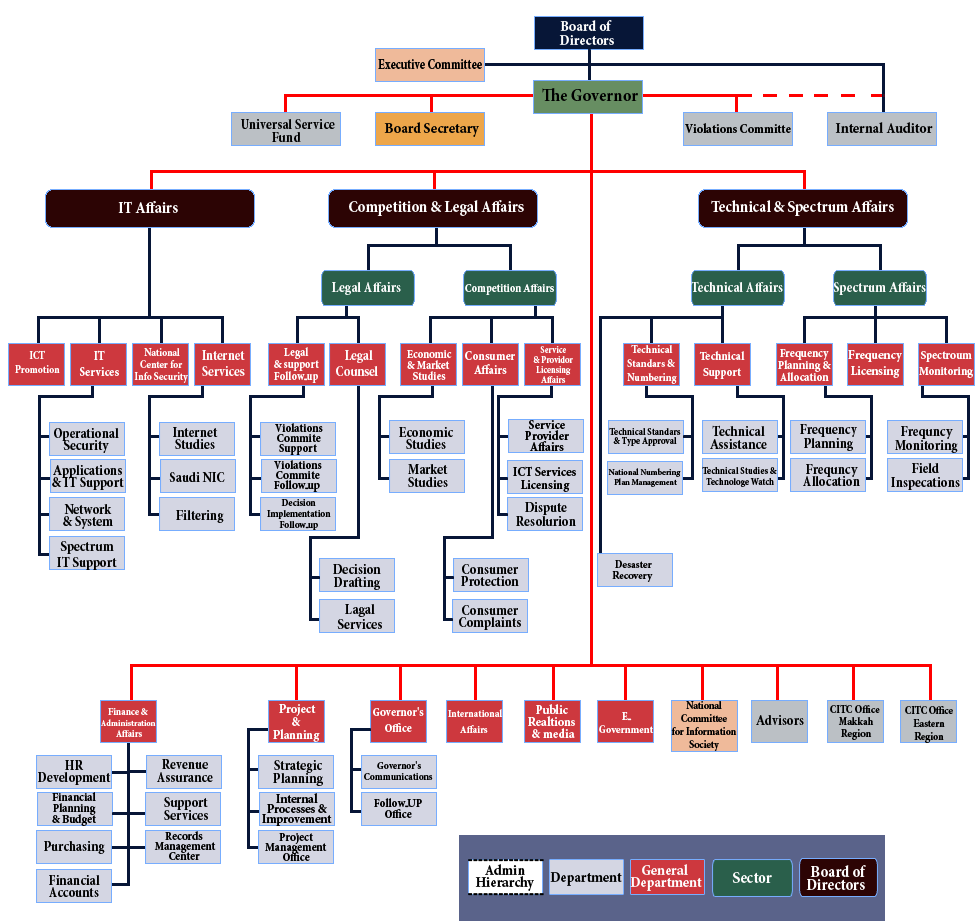
\includegraphics[width=.6\textwidth]{figures/citc2013organizational}
\caption{CITC organizational structure~\cite{citc2013organizational}}
\label{fig:citc2013organizational}
\end{figure}

Lastly, Figure~\ref{fig:johnson2012election} displays the 2012 american election
results between Barack Obama and Mitt Romney, with Obama being declared victor
by 332 votes to 206. This is a nominal set because there is no sense of ordering
here, with two people contending to be elected. It is possible to see the US
national territory and its states (another nominal set) with the number of votes
obtained by the winning candidate. The figure makes use of the following
Mackinlay attributes: position, color hue, connection, containment, shape,
length, and area.

\begin{figure}[H]
\centering
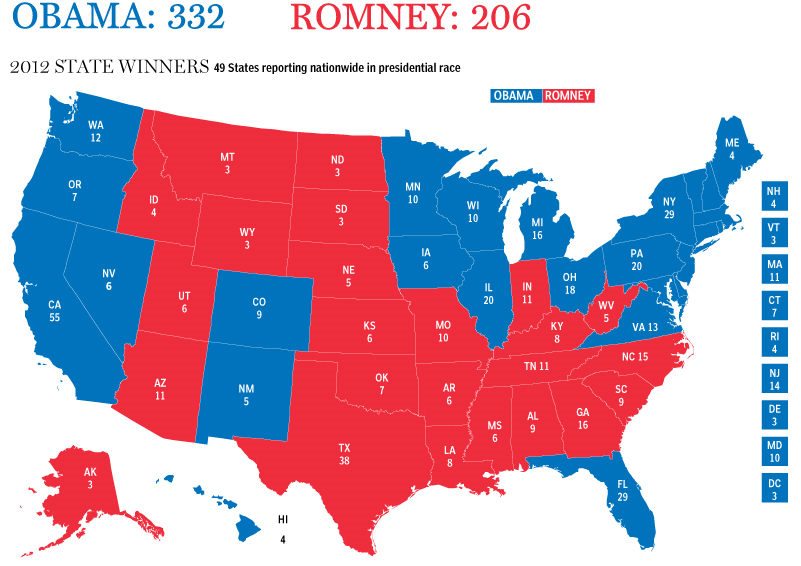
\includegraphics[width=.6\textwidth]{figures/johnson2012election}
\caption{U.S. 2012 election results~\cite{johnson2012election}}
\label{fig:johnson2012election}
\end{figure}

\subsection{Software visualization}

Considering software visualization as a discipline only concerned with the
visualization of algorithms and programs is a too-narrow definition. It is
necessary to widen it in a way where this term means \textit{the visualization
of artifacts related to software and its development process}.
These artifacts may not only be program code, but may also include requirements
and design documentation, changes in the source code, bug reports and, in the
scope of this research, coverage based debugging information, explained in
Section~\ref{sec:bg-debugging}.

In short, software visualization's objective is visualizing the structure,
behavior, and evolution of software~\cite{diehl2007software}. This field of
research is considered a specialization of information visualization---since
algorithms, files and lines of code in software systems are a kind of
information---whose goal is to help to comprehend software systems and to
improve the productivity of the software development process.

To achieve the previously stated objective, it is important to follow at least
one of the following principles.

\textit{Principle of interactive exploration:} This principle, also called The
Information Seeking Mantra~\cite{shneiderman1996eyes}, states that in order to
explore the data, interactive visualizations should allow the user to first get
an overview, and then zoom and filter, getting the details on demand.

\textit{Principle of Focus $+$ Context:} This principle states that a detailed
visualization of some part of the information---the focus---is embedded within a
visualization of the context. What it means is that techniques that cope with
this principle must provide both an overview and detail at the same time.

\section{Final remarks}

This chapter presented the fundamental concepts and techniques that form the
foundation for this research, providing the necessary background knowledge on
testing (Section~\ref{sec:bg-testing}), code coverage
(Section~\ref{sec:bg-codecoverage}), coverage based debugging
(Section~\ref{sec:bg-debugging}), and information visualization
(Section~\ref{sec:bg-infovis}). A more in-depth discussion on software
visualization will be presented in Chapter~\ref{ch:related}.
